\documentclass{beamer}
\usepackage{amsmath}
\usepackage{amssymb}
\usepackage{pgf}
\usepackage{tikz}
\usepackage{nicefrac}
\usepackage{listings}
\usepackage{color}
\usetikzlibrary{matrix}
\usetheme{boxes}
\newcommand{\fig}{figures} % common figure path
\newcommand{\dbbslsh}{\textbackslash \textbackslash} % common figure path
\newcommand{\frnzplt}{FranzPlot }
\newenvironment{myblock}[3]{%
\definecolor{smtbx}{rgb}{0.64,0.76,0.68}
\setbeamercolor{block body}{#2}
\setbeamercolor{block title}{#3}
\begin{block}{#1}}{\end{block}}
\title[Curve e Sup. - Lab 5]{Curve e Superfici per il Design \\ Laboratorio 5 - Curve parametriche}
\author[Prof.ssa Scotti]{Prof. Nicola Parolini}
%\institute[dimat]{Long Inst.}
\date{21 Novembre 2019}

\begin{document}
%\lstset{language=POV}
\begin{frame}
\maketitle
\end{frame}
\section{Introduzione}
\begin{frame}
\frametitle{Materiali}
Nella cartella con il materiale di oggi troverete:
\begin{itemize}
\item Questa presentazione \\ (\texttt{Materiale Didattico/Laboratori/lab 5/lab5\_testo.pdf});
%\item Il file \texttt{es\_dado\_ref.toml} con l'esercizio risolto della passata esercitazione.
\item L'eseguibile del \frnzplt \\ (\texttt{Software/Franzplot 19.08 - Windows.exe})
\end{itemize}
\end{frame}

\section{Riepilogo}
%
\begin{frame}
\frametitle{Esercizio 1: Curve con \frnzplt - Il comando parametric curve}
Sia data la seguente curva:
\begin{displaymath}
\mathcal C:
\begin{cases}
    x = \cos t\\
    y = 2 \sin t \\
    z = 0.5
\end{cases}
    \quad
    t \in [0, 2\pi]
\end{displaymath}
    Vogliamo rappresentarla con \frnzplt usando il nodo \texttt{Curve}.
\end{frame}
%

\begin{frame}
\frametitle{Esercizio 1 - i}
    Come avevamo visto nel caso del plot di rette, anche oggi faremo uso dei seguenti nodi:
    \begin{itemize}
        \item \texttt{Geometries > Curve} 
        \item \texttt{Parameters > Interval}
        \item \texttt{Geometry Renderer}
    \end{itemize}

    \vspace{0.5cm}
    A differenza della visualizzazione di una retta, questa volta sar\`a fondamentale assegnare i valori corretti
    all'inizio e la fine dell'intervallo.
\end{frame}
%
\begin{frame}
\frametitle{Esercizio 1 - ii}
\begin{center}
\begin{tikzpicture}
\node(img1){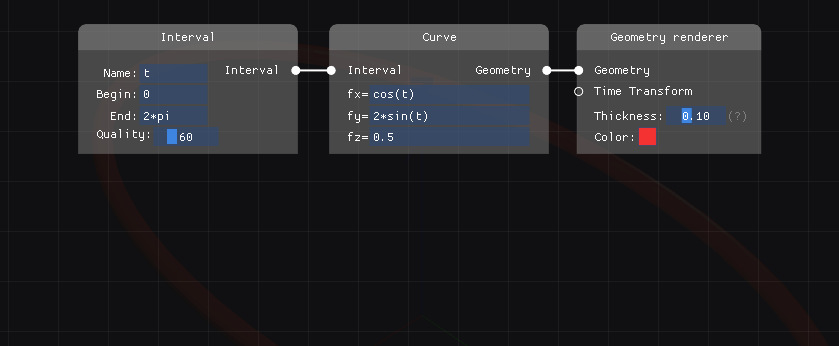
\includegraphics[width=0.8\textwidth]{\fig/lab5_es1_graph.png}};
\node(img2) at (img1.south){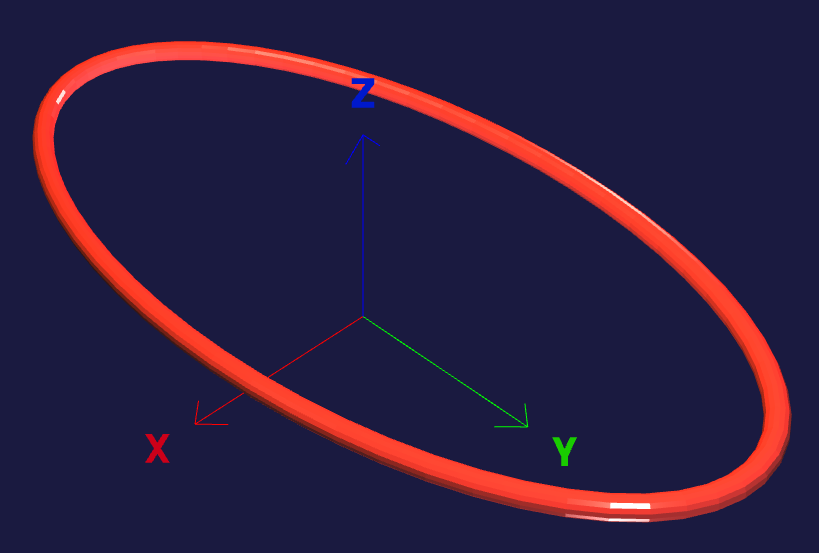
\includegraphics[width=0.5\textwidth]{\fig/lab5_es1_scene.png}};
\end{tikzpicture}
\end{center}
    Il parametro \texttt{Quality} indica quanti punti saranno usati dal \frnzplt per
    approssimare la curva (o la superficie)

\end{frame}
%%
\begin{frame}
\frametitle{Esercizio 2: Rotazione di un punto}

    Sia dato il punto $P(0, 1, 1)$.
    \begin{itemize}
        \item Scrivere la generica matrice $R$ di rotazione intorno l'asse Z.
        \item Applicare a $P$ una trasformazione parametrica di rotazione intorno l'asse Z, con parametro $\theta \in [0, \pi]$,
            e scrivere la curva parametrica ottenuta. Di che curva si tratta?
        \item Rappresentare il punto $P$ e la curva ottenuta in \frnzplt.
        \item Usando \frnzplt, disegnare la curva applicando al punto una matrice parametrica.
    \end{itemize}

\end{frame}

\begin{frame}
\frametitle{Esercizio 2 - i}
La matrice che rappresenta la trasformazione parametrica \`e la seguente:
\begin{equation*}
R(\theta) = 
\begin{bmatrix}
    \mbox{cos}(\theta) & - \mbox{sin}(\theta) & 0 & 0\\
    \mbox{sin}(\theta) & \mbox{cos}(\theta)   & 0 & 0\\ 
    0 & 0 & 1 & 0 \\
    0 & 0 & 0 & 1
\end{bmatrix}
\quad
    \theta \in [0, \pi]
\end{equation*}

    Per ottenere la curva dobbiamo moltiplicarla per il vettore che contiene le coordinate del punto: 
    $$
    c(\theta) = R(\theta) \ P
    $$
\end{frame}

\begin{frame}
\frametitle{Esercizio 2 - ii}
Svolgendo i conti troviamo:
\begin{equation*}
c(\theta) = 
\begin{bmatrix}
    \mbox{cos}(\theta) & - \mbox{sin}(\theta) & 0 & 0\\
    \mbox{sin}(\theta) & \mbox{cos}(\theta)   & 0 & 0\\ 
    0 & 0 & 1 & 0 \\
    0 & 0 & 0 & 1
\end{bmatrix}
\cdot
\begin{bmatrix}
    0 \\
    1 \\
    1 \\
    1
\end{bmatrix}
 = 
\begin{bmatrix}
    -sin(\theta) \\
    cos(\theta) \\
    1 \\
    1
\end{bmatrix}
\end{equation*}
Quindi possiamo scrivere la nostra curva:
\begin{displaymath}
    c(\theta):
\begin{cases}
    x = -sin(\theta) \\
    y = cos(\theta) \\
    z = 1 \\
\end{cases}
\quad
    \theta \in [0, \pi]
\end{displaymath}

Poich\'e $\theta$ varia da $0$ a $\pi$, la curva \`e una semicirconferenza.
\end{frame}

\begin{frame}
\frametitle{Esercizio 2 - iii}
\begin{center}
\begin{tikzpicture}
\node(img1){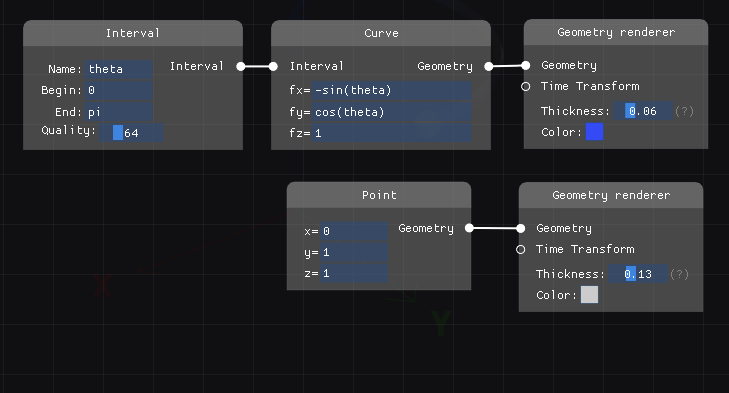
\includegraphics[width=0.8\textwidth]{\fig/lab5_es2_graph.png}};
\node(img2) at (img1.south west){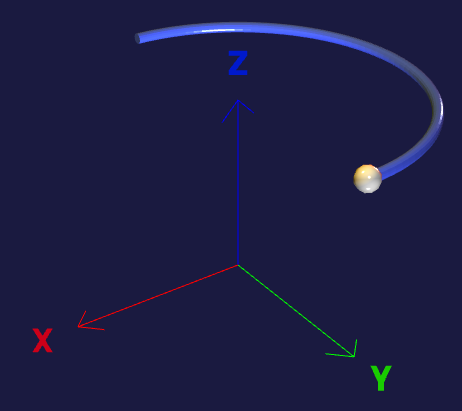
\includegraphics[width=0.4\textwidth]{\fig/lab5_es2_scene.png}};
\end{tikzpicture}
\end{center}

\end{frame}

\begin{frame}
\frametitle{Esercizio 2 - iv}
    Nel \frnzplt \`e possibile scrivere matrici parametriche e usare il nodo \texttt{Transform} per
    applicare una trasformazione parametrica a una geometria 0D o 1D (punto o curva).

    \begin{itemize}
        \item Nota: non \`e possibile applicare trasformazioni parametriche a primitive come cubi, dadi, ecc
    \end{itemize}

    \vspace{1cm}
    Per scrivere una trasformazione parametrica, \`e sufficiente usare il nodo
    \texttt{Generic Matrix}, collegare in input l'\texttt{Interval} del parametro da usare,
    e scrivere espressioni contenenti il parametro all'interno della matrice.

\end{frame}

\begin{frame}
\frametitle{Esercizio 2 - v}
\begin{center}
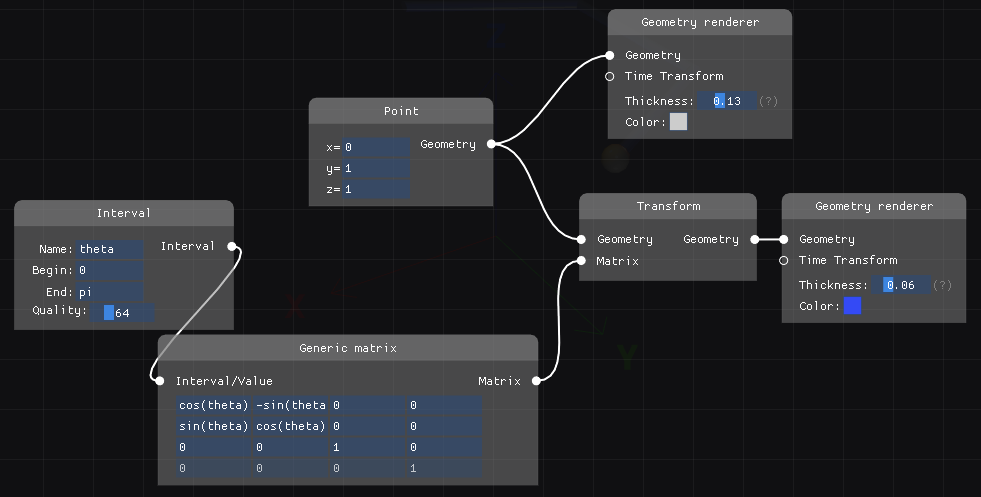
\includegraphics[width=\textwidth]{\fig/lab5_es2_param_transform.png}
\end{center}

    Come sempre il nome del parametro \`e arbitrario (\texttt{theta}, \texttt{t}, \texttt{r}, sono tutti validi).
    L'importante \'e essere \textbf{consistenti}.
\end{frame}
%
\begin{frame}
\frametitle{Esercizio 3}
    Sia data la seguente curva parametrica:
	\begin{displaymath}
	\mathcal{C}:\begin{cases}
	x(t)=  \nicefrac{1}{2} \ t \cos t\\
	y(t)= 0 \\
        z(t)= \nicefrac{1}{2} \ t \sin t
	\end{cases}
	\qquad 0 \leq t \leq 10 \pi
	\end{displaymath}
    \begin{itemize}
        \item Dire di che tipo di curva si tratta.
        \item Scrivere la matrice di scalatura $S$ che abbia parametri di scalatura $S_x = \nicefrac{1}{4}$, $S_y = 1$, $S_z = \nicefrac{1}{2}$.
        \item Calcolare la curva $\mathcal{G}$ ottenuta applicando la trasformazione $S$ a $\mathcal{C}$.
        \item Rappresentare le curve $\mathcal{C}$ e $\mathcal{G}$ in \frnzplt.
        \item Verificare con \frnzplt il risultato ottenuto, applicando la trasformazione $S$ a $\mathcal{C}$.
    \end{itemize}
\end{frame}

\begin{frame}
\frametitle{Esercizio 3 - i}
Scriviamo la matrice di scalatura richiesta:
\begin{equation}
S = 
\begin{bmatrix}
    \nicefrac{1}{4} &       0 & 0\\
    0  & 1 & 0\\ 
    0 & 0 & \nicefrac{1}{2} 
\end{bmatrix}
\end{equation}
    Trattandosi di una scalatura, \`e immediato calcolare la curva $\mathcal{G}$ \\
    (\`e sufficiente moltiplicare ogni espressione in $x$, $y$ e $z$ per la corrispondente scalatura).
\begin{displaymath}
    \mathcal{G}(t):
\begin{cases}
    x = \nicefrac{1}{8} \ t \cos t \\
    y = 0 \\
    z = \nicefrac{1}{4} \ t \sin t
\end{cases}
\quad
    t \in [0, 10 \pi]
\end{displaymath}

\end{frame}

\begin{frame}
\frametitle{Esercizio 3 - ii}
In alternativa, ricaviamo $\mathcal G$ come moltiplicazione di $S$ per $\mathcal C$:
\begin{displaymath}
    \mathcal G(t) = S \ \mathcal C(t)
\end{displaymath}

\begin{displaymath}
    \mathcal G = 
\begin{bmatrix}
    \nicefrac{1}{4} &       0 & 0 & 0\\
    0  & 1 & 0 & 0 \\ 
    0 & 0 & \nicefrac{1}{2} & 0 \\
    0 & 0 & 0 & 1
\end{bmatrix}
\begin{bmatrix}
    \nicefrac{1}{2} t \cos t \\
    0 \\
    \nicefrac{1}{2} \ t \sin t \\
    1
\end{bmatrix}
 =
\begin{bmatrix}
    \nicefrac{1}{8} \ t \cos t \\
    0 \\
    \nicefrac{1}{4} \ t \sin t \\
    1
\end{bmatrix}
\end{displaymath}

    \vspace{0.7cm}
Possiamo notare come in questo esercizio il parametro della curva $\mathcal G$ ``deriva'' dalla curva che stiamo trasformando,
    mentre nell'esercizio precedente, il parametro ``deriva'' dalla matrice parametrica, non dal punto che abbiamo trasformato.
\end{frame}

%
\begin{frame}
\frametitle{Esercizio 3 - iii}
\begin{center}
\begin{tikzpicture}
\node(img1){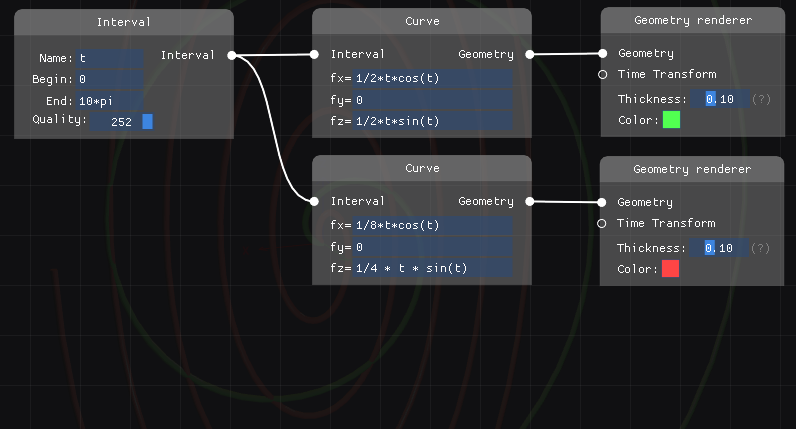
\includegraphics[width=0.8\textwidth]{\fig/lab5_es3_graph.png}};
\node(img2) at (img1.south west){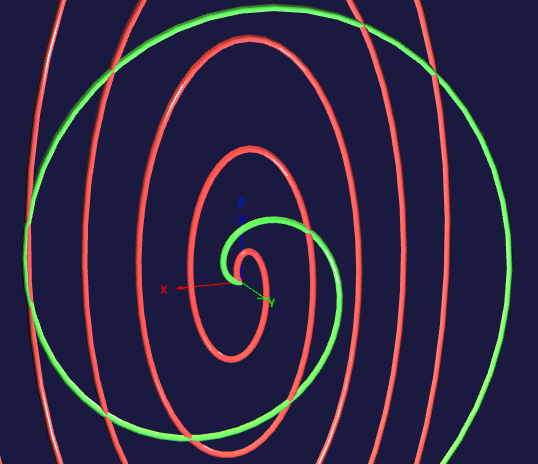
\includegraphics[width=0.5\textwidth]{\fig/lab5_es3_scene.png}};
\end{tikzpicture}
\end{center}
    Poich\`e l'intervallo \`e parecchio ampio, si suggerisce di settare il parametro \texttt{Quality} al massimo.
\end{frame}

\begin{frame}
	\frametitle{Esercizio 4 - Sole/Terra/Luna}
	L'equazione parametrica della circonferenza (di raggio $a$):
	\begin{displaymath}
	\mathcal{C}:\begin{cases}
	x(t)= a \cos t\\
	y(t)= a \sin t\\
	z(t)= 0
	\end{cases}
	\qquad 0 \leq t \leq 2 \pi
	\end{displaymath}
	\`e utile anche per descrivere l'orbita dei corpi celesti.
	\begin{itemize}
		\item Ponendo il Sole al centro del sistema di riferimento, scrivere le curve che descrivono il moto della Terra e della Luna rispetto al Sole e rappresentarle su \frnzplt.
		\item Rappresentare il sistema Sole/Terra/Luna utilizzando punti e/o sfere e l'elemento \texttt{Time Transform}.
	\end{itemize}
\end{frame}

\begin{frame}
	\frametitle{Esercizio 4 - i}
	\begin{block}{Suggerimento}
		Per ogni valore del parametro t, il moto della Luna rispetto al Sole pu\`o essere visto come:
		\begin{displaymath}
		\mathcal{C}_{LS}:\begin{cases}
		x(t)= x_{TS}(t) + x_{LT}(t) \\
		y(t)= y_{TS}(t) + y_{LT}(t)\\
		z(t)= 0
		\end{cases}
		\end{displaymath}
		dove $x_{TS}(t)$ e $y_{TS}(t)$ indicano il moto della Terra rispetto al Sole, mentre 
		$x_{LT}(t)$ e $y_{LT}(t)$ indicano il moto della Luna rispetto alla Terra.

                Non dimentichiamoci che la Luna ruota intorno alla Terra molto pi\`u velocemente di quanto la Terra ruoti intorno al sole!\\
                (Circa 1 mese vs 1 anno)
	\end{block}
\end{frame}

\begin{frame}
\frametitle{Esercizio 4 - risultato}
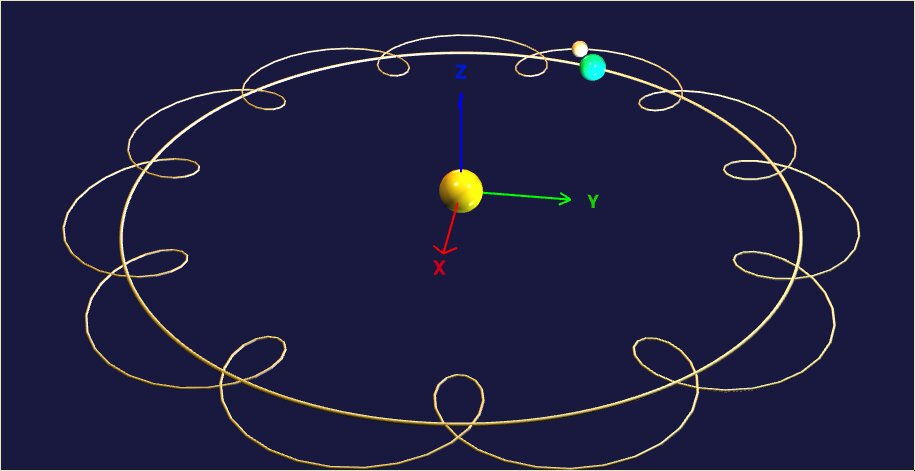
\includegraphics[width=\textwidth]{\fig/sunsys.jpeg}
\end{frame}

\begin{frame}
	\frametitle{Esercizio 4 - ii}
	
	\begin{columns}
		\begin{column}{0.5\textwidth}
			Se si indica con $R$ il raggio della circonferenza sulla quale la Terra si muove rispetto al Sole, l'equazione per descrivere il suo moto rispetto al Sole \`e:
			\begin{displaymath}
			\mathcal{C}_{TS}:\begin{cases}
			x_{TS}(t)= R \cos(t)\\
			y_{TS}(t)= R \sin(t)\\
			z_{TS}(t)= 0
			\end{cases}
			\end{displaymath}
		\end{column}
		\begin{column}{0.5\textwidth}
			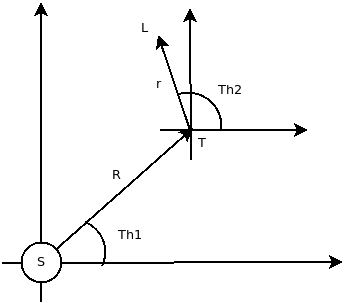
\includegraphics[width=.8\textwidth]{\fig/ex_sun_earth_moon.png}
		\end{column}
	\end{columns}
\vspace{0.2cm}
    Allo stesso modo, indicando con $r$ il raggio della circonferenza sulla quale la Luna si muove rispetto alla Terra,  l'equazione per descrivere il suo moto rispetto alla Terra (cio\`e se abbiamo la Terra all'origine degli assi), \`e:
	\begin{displaymath}
	\mathcal{C}_{LT}:\begin{cases}
	x_{LT}(t)= r \cos(kt)\\
	y_{LT}(t)= r \sin(kt)\\
	z_{LT}(t)= 0
	\end{cases}
	\end{displaymath}
\end{frame}

\begin{frame}
\frametitle{Esercizio 4 - iii}

\begin{columns}
\begin{column}{0.5\textwidth}
Questo ci permette di esprimere la posizione della Luna nel sistema di riferimento del Sole come la posizione della Terra rispetto al Sole  pi\`u la posizione della Luna rispetto alla Terra (come suggerito):
\end{column}
\begin{column}{0.5\textwidth}
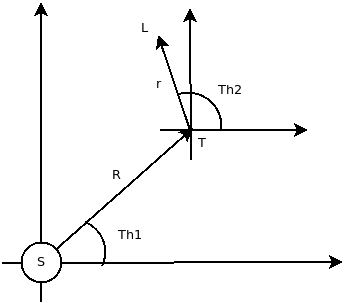
\includegraphics[width=.8\textwidth]{\fig/ex_sun_earth_moon.png}
\end{column}
\end{columns}
\vspace{0.4cm}
\begin{displaymath}
\mathcal{C}_{LS}:\begin{cases}
 x(t)=  R \cos(t) + r \cos(kt)\\
 y(t)=  R \sin(t) + r \sin(kt)\\
 z(t)= 0
\end{cases}
\qquad 0 \leq t \leq 2 n \pi
\end{displaymath}
dove $n =$ numero rivoluzioni della Terra attorno al Sole. \\
\vspace{0.2cm}
\textbf{Oss.} Poich\`e si vuole che la Luna ruoti pi\`u velocemente della Terra dev'essere necessariamente $k > 1$. In questo modo per una stessa $t$ la Luna avr\`a spazzato un angolo maggiore.
\end{frame}


\begin{frame}
	\frametitle{Esercizio 4 - iv} 
	\begin{itemize}
	\item Note le espressioni delle curve $\mathcal{C}_{TS}$ e $\mathcal{C}_{LS}$, non rimane che
	decidere le lunghezze dei due raggi (per i quali, per ottenere un risultato
	realistico, vorremmo $r<R$), e il valore di $k$.  
	\item $k = 12$, ad esempio, \`e un valore realistico poich\'e come suggerito, il periodo di rivoluzione lunare \`e circa 1 mese, mentre il periodo di rivoluzione terrestre \`e circa un anno. Quindi la velocit\`a di rotazione della Luna sar\`a circa 12 volte pi\`u grande di quella della Terra.
	\end{itemize}
\end{frame}


\begin{frame}
	\frametitle{Esercizio 5 - Spirale conica}
	
	\begin{center}
		\begin{tikzpicture}
		\node(img1){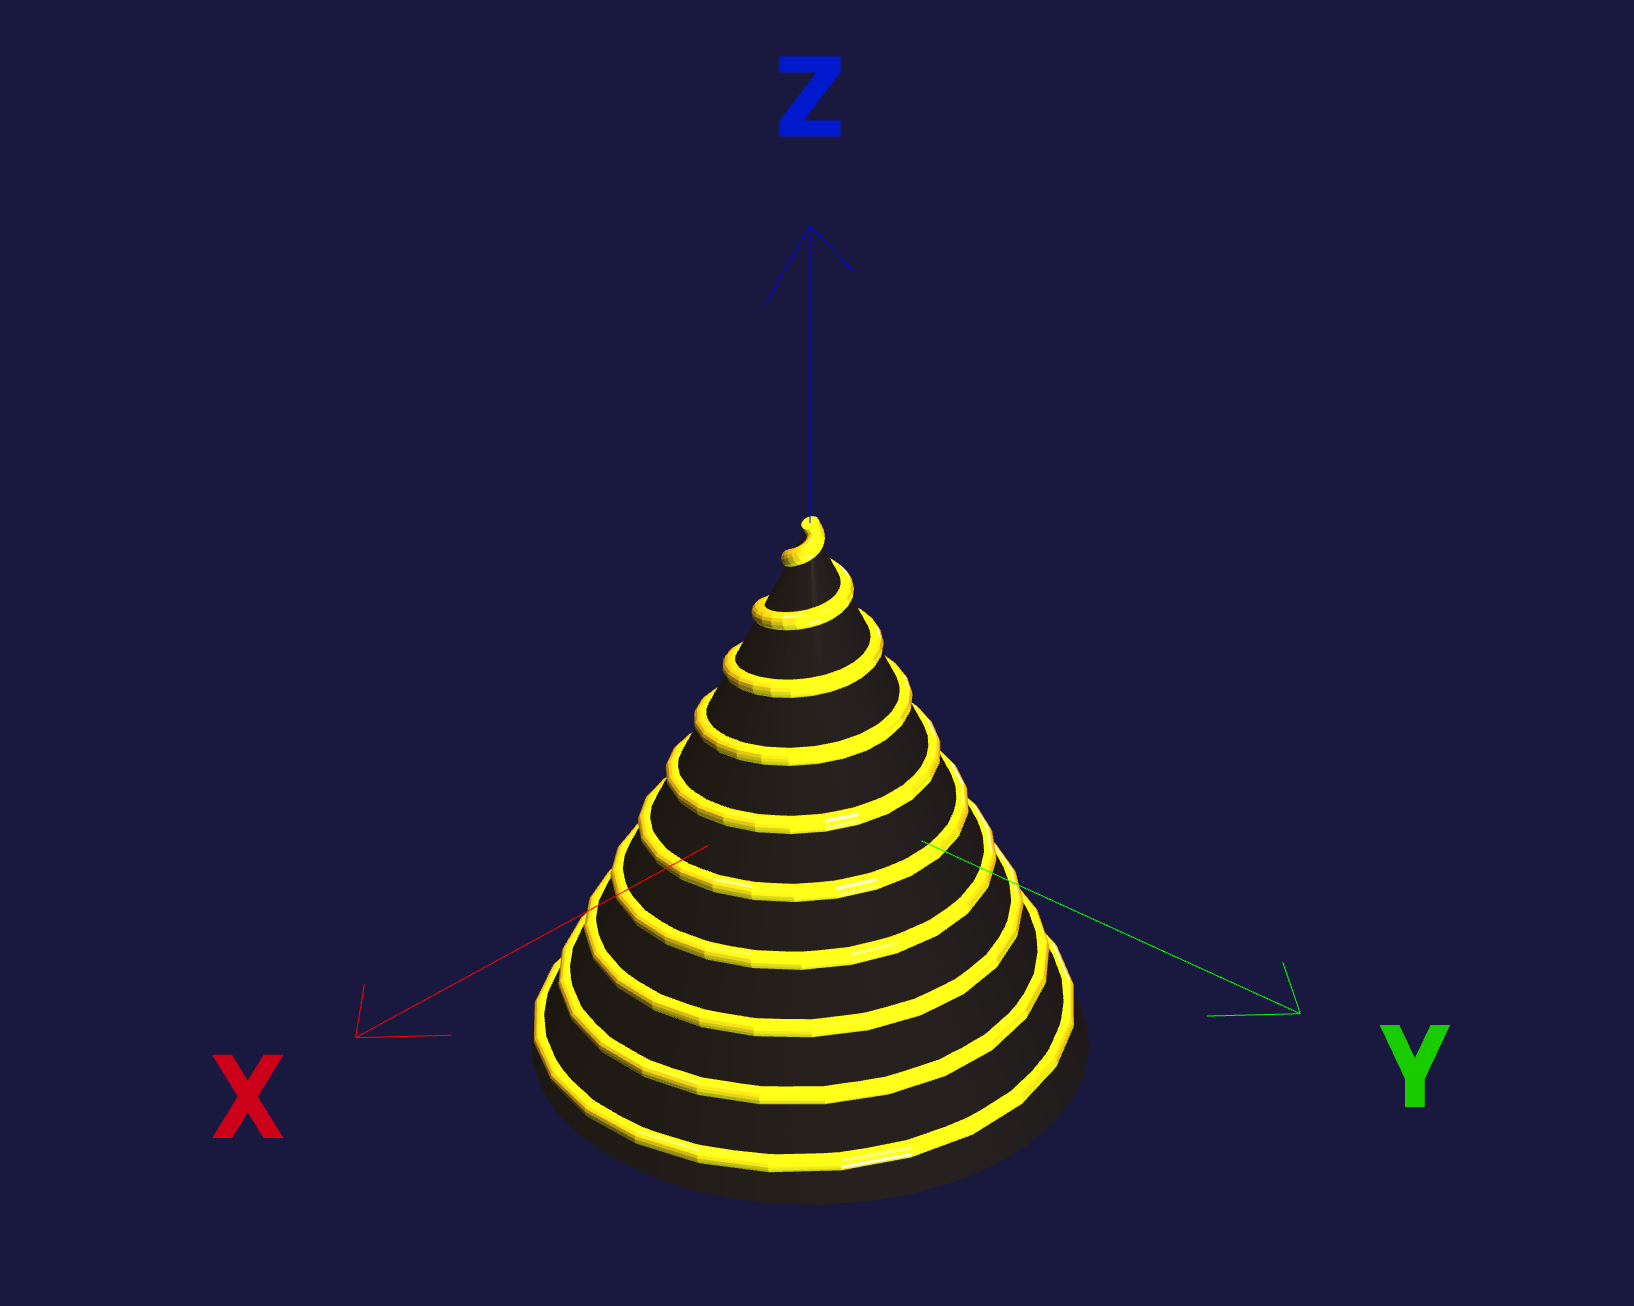
\includegraphics[width=.65\textwidth]{\fig/l4_cone_helix}};
		\end{tikzpicture}
	\end{center}
	Determinare la curva parametrica che descrive il filo avvolto sul cono (ottenuto da \texttt{Geometries $\rightarrow$ Primitive} con \texttt{Size} $=1$). 
\end{frame}

\begin{frame}
	\frametitle{Esercizio 5 - i}
La curva \`e data dalla rotazione di un punto intorno all'asse, con raggio
variabile, composta con una traslazione lungo lo stesso asse, quindi si tratta
di un'elica conica, con valori di $t$ negativi perch\`e vogliamo il tratto inferiore dell'elica conica.
	\begin{displaymath}
	\mathcal{C}:\begin{cases}
	x(t)= at\cos t\\
	y(t)=at \sin t\\
	z(t)= ct + d
	\end{cases}
	\qquad -2 n \pi \leq t\leq 0
	\end{displaymath}
	
        Chiamiamo $h_z = 2 \pi c$ il passo dell'elica in direzione z e $h_{r} = 2 \pi a$ il passo dell'elica in direzione radiale.
\end{frame}

\begin{frame}
	\frametitle{Esercizio 5 - ii}
        Dobbiamo determinare i parametri $a$, $c$, $n$, $d$ che ci diano il giusto passo in direzione radiale, passo in direzione z,
        numero di avvolgimenti e traslazione lungo z dell'elica.
	\begin{itemize}
		\item Affinch\'e la punta della spirale e del cono coincidano, devo traslare l'origine degli assi e portarla sulla punta del cono. La punta del
                    cono ha coordinate $P(0, 0, 0.5)$, quindi $d = 0.5$.
		\item Il numero di avvolgimenti dell'elica $n$ pu\`o essere dedotto dalla figura dell'esercizio. Quindi $n = 10$.
	\end{itemize}
\end{frame}

\begin{frame}
	\frametitle{Esercizio 5 - iii}
	\begin{itemize}
		\item Il passo in direzione z dell'elica moltiplicato per il numero di avvolgimenti \`e pari all'altezza del cono, nel nostro caso 1. Quindi:
	\end{itemize}
                \begin{gather*}
		h_z n = 1 \Rightarrow 2 \pi c n = 1  \\
                c = \frac{1}{2 \pi n} = \frac{1}{20 \pi}
                \end{gather*}
	\begin{itemize}
		\item Il passo in direzione radiale dell'elica moltiplicato per il numero di avvolgimenti dà il raggio del cono, che è pari a 0.5. Quindi:
	\end{itemize}
		\begin{align*} 
		h_r n = 0.5 \Rightarrow 2 \pi a n = 0.5 \\
                    a = \frac{1}{4 \pi n} = \frac{1}{40 \pi}
		\end{align*}
\end{frame}

\begin{frame}
	\frametitle{Esercizio 5 - iv}
        Andando a sostituire trovo l'equazione parametrica cercata:
	\begin{displaymath}
	\mathcal{C}:\begin{cases}
            x(t)= \nicefrac{1}{(40\pi)}t \cos t\\
            y(t)= \nicefrac{1}{(40\pi)}t \sin t\\
            z(t)= \nicefrac{1}{(20\pi)}t + 0.5
	\end{cases}
	\qquad -2 n \pi \leq t\leq 0
	\end{displaymath}

        \textbf{NOTA:} Per rappresentare la curva in \frnzplt, impostare la \texttt{Quality} dell'intervallo al massimo valore consentito.
	
        \vspace{0.5cm}
	\begin{itemize}
                \item
		\textbf{Oss.} Sfruttando la similitudine tra triangoli \`e possibile dedurre che il rapporto
                tra raggio e altezza del cono \`e pari al rapporto tra passo in direzione radiale e in z dell'elica. Nel nostro caso:
		\begin{displaymath}
			\frac{R_C}{H_C} = \frac{h_r}{h_z} = \frac{a}{c} = \frac{1}{2}
		\end{displaymath}
	\end{itemize}
\end{frame}


\end{document}
